% Template for PLoS
% Version 1.0 January 2009
%
% To compile to pdf, run:
% latex plos.template
% bibtex plos.template
% latex plos.template
% latex plos.template
% dvipdf plos.template

\documentclass[10pt]{article}

% amsmath package, useful for mathematical formulas
\usepackage{amsmath}
% amssymb package, useful for mathematical symbols
\usepackage{amssymb}

% graphicx package, useful for including eps and pdf graphics
% include graphics with the command \includegraphics
\usepackage{graphicx}

% cite package, to clean up citations in the main text. Do not remove.
\usepackage{cite}

\usepackage{color} 

% Use doublespacing - comment out for single spacing
%\usepackage{setspace} 
%\doublespacing

\newcommand{\argmin}{\operatornamewithlimits{argmin}}

% Text layout
\topmargin 0.0cm
\oddsidemargin 0.5cm
\evensidemargin 0.5cm
\textwidth 16cm 
\textheight 21cm

% Bold the 'Figure #' in the caption and separate it with a period
% Captions will be left justified
\usepackage[labelfont=bf,labelsep=period,justification=raggedright]{caption}

% Use the PLoS provided bibtex style
\bibliographystyle{plos2009}

% Remove brackets from numbering in List of References
\makeatletter
\renewcommand{\@biblabel}[1]{\quad#1.}
\makeatother


% Leave date blank
\date{}

\pagestyle{myheadings}
%% ** EDIT HERE **


%% ** EDIT HERE **
%% PLEASE INCLUDE ALL MACROS BELOW

%% END MACROS SECTION

\begin{document}

% Title must be 150 characters or less
\begin{flushleft}
{\Large
\textbf{Metagenome phylogeny for the 1\%}
}
% Insert Author names, affiliations and corresponding author email.
\\
Aaron E. Darling$^{1,\ast}$,
Guillaume Jospin$^{1}$, 
Holly M. Bik$^{1}$,
Jonathan A. Eisen$^{2,3}$
\\
\bf{1} Genome Center, University of California-Davis, California, United States of America
\\
\bf{2} Department of Evolution and Ecology, University of California-Davis, California, United States of America
\\
\bf{3} Department. of Medical Microbiology and Immunology, University of California-Davis, California, United States of America
\\
$\ast$ E-mail: aarondarling@ucdavis.edu
\end{flushleft}

% Please keep the abstract between 250 and 300 words
\section*{Abstract}
blahdeeblah, blah blah
% Please keep the Author Summary between 150 and 200 words
% Use first person. PLoS ONE authors please skip this step. 
% Author Summary not valid for PLoS ONE submissions.   
\section*{Author Summary}

\section*{Introduction}

From the human microbiome to marine ecosystems, metagenomic approaches have revolutionized biology. High-throughput sequencing has rapidly revealed the vastness of uncharacterized microbial diversity and offereed an important first glimpse into the genetic structure of uncultured microbial communities.
However, in its current form, metagenomics destroys some of the most valuable information present in a sample: genetic linkage. 
Loss of information occurs in two ways: during sample extraction and size selection of fragments for sequencing.
In nearly all metagenomic sample processing methods, cells from the microbial community are lysed together to obtain a common pool of DNA.
This practice causes DNA from many different cells to mix together, so that the cellular compartmentalization of individual genotypes is destroyed.
Subsequently, long chromosome-scale DNA fragments are typically broken by mechanical or enzymatic means into fragments small enough for processing with current sequencing chemistries. 
The resulting sequenced fragments are usually less than 1Kbp (though sometimes 10-20kbp). 
Such shearing results in further loss of  genetic linkage information, since this method removes our ability to infer how short DNA fragments were arranged into chromosome-scale molecules.

Metagenomic approaches ultimately aim to characterize ecosystem function, and thus knowledge of individual genomes (including taxonomic classification and functional potential) will be imperative for piecing together our understanding of microbial assemblages.
Metagenomics methods are gaining increasingly widespread appeal.
They can be used to test longstanding biological hypotheses (is Everything Everywhere?) as well as offer practical applications such as in in microbial forensics ("fingerprinting" microbial communities, tracking and detecting biological agents).
Direct high-throughput sequencing of microbial communities has many advantages over culture-based methods, avoiding potential contamination, population bottlenecking, and taxonomic bias that is inherent to such studies.
In practice, improved sample processing methods could potentially retain the genetic linkage information of a microbial community throughout the sequencing process.
High throughput single-cell genomics (e.g. applied to thousands of cells) offers an alternative to the standard metagenomics workflow that preserves information about the compartmentalization of genetic material into cells. 
However, single-cell genomics currently presents its own challenges, associated with isolating individual cells from certain types of samples and amplifying the {DNA} from a single cell to attain the minimum quantity required for sequencing. 
Single-cell approaches also have extensive equipment requirements and are highly sensitive to contamination by foreign DNA, requiring rigorous laboratory and reagent decontamination. 
Furthermore, the interpretation and downstream analysis of single-cell data is complicated by empirical methodology (uneven amplification, sequence chimeras) and computational pipelines that are not yet optimized for single-cell genome assembly; in some cases shotgun metagenomic approaches may result in more extensive genome coverage and a less fragmented view of a given microbial genome ~\cite{Stepanauskas2012}. 

Given the current empirical limitations, practitioners most often resort to computational methods for reconstructing the genetic architecture of a microbial community after sequencing. 
Molecular evolution, the joint processes of DNA replication with mutation and natural selection acting on those mutations, provides the primary signal for most metagenome analysis methods. 
As species diverge, differences such as nucleotide substitutions, insertions, deletions, and genomic rearrangements accumulate in their genomes, and these differences can be leveraged to infer a sequence's origin in a mixed metagenomic sample.
Computational methods have so far demonstrated substantial promise for metagenomic analysis, with a wide range of approaches explored to date. 
Previous work has typically focused on a number of central problems, including taxonomic classification of sequences, estimation of community structure and relative abundances of organisms, and "binning" approaches that sort sequences into groups corresponding to some meaningful characteristic. 
Each of these issues are interrelated, and many computational methods attempt to simultaneously address two or more of these problems.

\subsection*{Previous work}

\subsubsection*{Whole metagenome binning}
Approaches for binning metagenomic reads fall into two categories: composition classifiers and identity/homology classifiers. 
Composition classifiers utilize the properties of the sequences themselves (e.g. GC content or oligonucleotide frequency) to bin nucleotide data into distinct groups, with the assumption that these characteristics contain useful phylogenetic signals~\cite{Campbell1999}~\cite{Karlin1997}. 
Each "bin" aims to encapsulate a distinct taxonomic entity or putative gene family, meaning that sequence fragments placed into the same group could be interpreted to have similar genomic features (and potentially represent linkage in the case of taxonomic bins). 
Existing composition classifiers include TACOA (supervised classification using k-nearest neighbors) ~\cite{Diaz2009}, PhyloPythia  ~\cite{Mchardy2006} and PhyloPythiaS (multiclass support vector machine classifier using oligonucleotide frequencies) ~\cite{Patil2011}, and Eu-Detect (oligonucleotide binning to separate eukaryote sequences in feature vector space) ~\cite{Mohammed2011}. 
Additional methods such as Self-Organizing Maps (e.g. eSOMS ~\cite {Dick2009}) utilize tetranucleotide frequencies in combination with read abundance information to produce visual "maps" displaying different bins. 

Alternatively, binning methods can compare metagenome reads against reference databases to obtain sequence identity information and putative homology. 
Popular tools for identity/homology classification include MEGAN (a Lowest Common Ancestor algorithm that summarizes BLAST outputs to assign taxonomy)~\cite{Huson2007}, SORT-Items (reciprocal BLAST approach to detect significant orthology)~\cite{Haque2009}, NBC (Naive Bayesian Classifier)~\cite{Rosen2011}, MTR (a variation on Lowest Common Ancestor approaches that uses multiple taxonomic ranks)~\cite{Gori2011}, and ProViDE (analysis of alignment parameter thresholds, specifically customized for classifying viral sequences)~\cite{Ghosh2011}.

Each type of binning method has benefits and drawbacks. 
Composition classifiers are arguably less biased because they can often analyze a larger proportion of metagenome data (versus methods that search for orthologous genes and/or rely on reference databases of known sequences). 
However, composition-based methods can become less useful for classifying complex environmental samples (increased noise results in lower low taxonomic resolution). 
Identity/homology binning methods can be more intuitive for investigating biological patterns, being easier to apply and resulting in more informative data outputs (e.g. hierarchical taxonomy).  
However, BLAST-based approaches are notorious ambiguous; sequence identity does not incorporate underlying models of evolution (unlike phylogeny-based approaches), and thus does not necessarily return the closest relative from a group of database sequences. 
In addition, novel sequences often return ambiguous classifications or no match at all, particularly if no close relative is present amongst reference database sequences. 
In any case, the incompleteness of reference databases often becomes a limiting factor in metagenome sequence analysis. 

\subsubsection*{Estimating community composition from amplicon data}
High-throughput sequencing methods often leverage information from marker gene amplicons (orthologous loci such as 16S/18S rRNA) to infer microbial community structure. 
In contrast to shotgun metagenomics, amplicon approaches can potentially offer deeper views (deeper sequencing that captures information from rare taxa) and require less starting genomic material because of the inherent requirement of PCR amplification. 
Since rRNA surveys offer a  "standardized" snapshot of microbial communities compared to metagenome sequencing (information from a single genetic locus, often utilizing common primer sets and hypervariable regions across studies), amplicon studies most often focus on the characterization and comparison of microbial communities, both within and between samples. 

A variety of software pipelines can be used to process and analyze rRNA amplicon data ~\cite{Bik2012}. 
Inferring microbial assemblages typically relies on clustering of Operational Taxonomic Units (e.g. at a 97\% sequence identity cutoff, using either de novo or reference-based clustering), where taxonomy is assigned to representative sequences using either BLAST searches or the RDP classifier (a Naive Bayesian Classifier ~\cite{Wang2007} ).
Users can subsequently carry out a suite of downstream ecological and diversity analyses, including rarefaction (e.g. analyses for Chao1 estimation, OTU richness, or phylogenetic diversity as implemented in QIIME ~\cite{Caporaso2010}), and Principal Component Analysis and Jackknife cluster analysis (e.g. using phylogeny-derived UniFrac distances ~\cite{Lozupone2005}).

Amplicon approaches are now cheap and relatively easy to carry out. 
However, while it is currently possible to get a consistent, broad-scale view of biological patterns across microbial assemblages, there are many computational bottlenecks hindering fine-scale analysis of amplicon data. 
Bioinformatic pipelines are not effectively able to separate the "rare biosphere" from low-quality data resulting from sequencing errors or chimeric reads ~\cite{Bik2012}. 
BLAST-based approaches are also not ideal for conveying accurate taxonomic analyses at the strain or species level, particularly for ecologically important groups with sparse coverage in reference database. 
Many amplicon studies use BLAST searches to specifically assess whether or not certain groups of taxa (often biological species) are present within a community assemblage. 
Such methods do not convey information about evolutionary relationships between taxa in a sample, nor do they account for potential multiple "best hits". 
While the RDP classifier ~\cite{Wang2007} provides a statistical method for assessing confidence in BLAST results, for biologists there is often no substitute for inspecting environmental sequence data within a phylogenetic tree.
Because this exploration is currently carried out manually, there is a pressing need for scaleable, computationally robust tree-based methods for high-throughput datasets.

Despite the ongoing challenges, the nature of ribosomal locus (conserved and slowly evolving) and its long use in phylogenetic studies has made such datasets ideal for analysis within a reference guide tree topology  (e.g. pplacer ~\cite{Matsen2010} ). 
Although short sequence lengths and heavy computational requirements have previously hindered the application of explicitly phylogenetic approaches for high-throughput sequence data, software pipelines such as QIIME ~\cite{Caporaso2010} are now beginning to support the phylogenetic placement approaches for rRNA amplicon data.  
The move towards such phylogenetic approaches will clarify biological insights from large amplicon datasets, conveying lineage-specific information and allowing more detailed comparisons of taxon abundance and microbial community structure.
      
\subsubsection*{Community composition from metagenomes}

Similar to amplicon studies, shotgun metagenomic approaches are now incorporating "phylogenomic" approaches classify metagenome reads and analyze microbial community composition. 
These approach focus on a small subset of phylogenetically-informative marker genes mined from metagenomic sequence reads, typically representing ~1\% of any given shotgun dataset (citation here?). 
Marker genes can either be well-characterized protein coding genes (e.g. ribosomal proteins or elongation factor genes) or conserved noncoding regions (e.g. rRNA); these are typically used to build reference databases and multiple sequence alignments, which are subsequently used to scan and mine input metagenome data. 
A wide variety of computational approaches are now available to investigate the community composition of metagenome datasets, including: AMPHORA (bacterial protein markers and tree insertion via parsimony) ~\cite{WuEisen2008} and AMPHORA2 (bacterial/archael protein and DNA markers and tree insertion via likelihood or parsimony) ~\cite{Wu2012}, MLTreeMap (reference gene families with taxonomic and functional information and tree insertion via maximum likelihood) ~\cite{Stark2010}, MetaPhyler (taxonomic classifiers for each of the reference marker genes published in the AMPHORA set) ~\cite{Liu2010}, MetaPHlan (a taxonomic classifier harnessing fast search steps to mine clade-specific marker genes and estimate microbial taxon abundance)~\cite{Segata2012}, PhymmBL (a taxonomic classifier that combines sequence composition information with BLAST approaches)  ~\cite{Brady2009} ~\cite{Brady2011}, EMIRGE (iterative mapping method to reconstruct rRNA genes from metagenome data and estimate taxon abundance)~\cite{Miller2011}, and PhylOTU (probabilistic models used to mine rRNA and define OTUs from metagenome data)\cite{Sharpton2011}

Estimating microbial community composition from metagenome data is advantageous because it avoids any taxonomic bias that may be introduced through the use of PCR primers in amplicon studies. 
Metagenome surveys have the potential to provide much deeper insight, although the phylogenetic breadth of reference genome databases remains much more limited relative to marker genes (e.g. rRNA). 
Community composition and relative organism abundance can additionally be estimated in conjunction with functional information derived from genomic data, providing a more complete snapshot of microbial assemblages. 
In contrast to computational pipelines for amplicon data, software tools for metagenome data have rapidly moved towards phylogeny-based frameworks and use of more statistically robust algorithms (e.g. using probabilistic models to create profile sequence alignments, containing information about positional homology and secondary structure in the case of rRNA genes). 
Recent improvements in computational requirements has increasingly facilitated the adoption of such probabilistic methods in metagenome analysis.
For example, AMPHORA ~\cite{WuEisen2008}, AMPHORA2 ~\cite{Wu2012}, and MLTreeMap ~\cite{Stark2010} incorporate the use of profile Hidden Markov Models (HMMs) via the HMMer software suite ~\cite{Eddy2011}, while PhylOTU ~\cite{Sharpton2011} relies on covariance models for rRNA as implemented in the INFERNA ~\cite{Nawrocki2009}. 
Unlike the scoring system used in BLAST, probabilistic models relay confidence values by reporting the most probable state amongst all choices (e.g. the best alignment that can be predicted for a given sequence). 

***Maybe one or two more summary sentences here - what is the take home message about why we should use HMMs? What are the potential disadvantages that we have to keep in mind (e.g. complications arising when you have profile alignments containing divergent sequences)***

In the present manuscript, we introduce PhyloSift, a new method for reconstructing the genetic architecture of a metagenomic sample and for comparison of community structure among multiple related samples.
The new method leverages explicitly phylogenetic models of molecular evolution to provide high resolution detection of organisms in a metagenome. 
Our approach is based on well known statistical phylogenetic models, is amenable to Bayesian hypothesis testing, and uses name-independent analyses to provide higher resolution about microbial community assemblages (versus methods that rely on taxonomy). This method can be applied to any single phylogeny at a time.
We additionally propose a set of 40 "elite" marker gene families that have largely congruent phylogenetic histories, thus improving the limit of detection for rare organisms.
We contribute an open-source implementation of the method that has been engineered for ease-of-use on 64-bit Linux and Mac platforms.
Finally, we compare the features of PhyloSift to some related methods to provide readers with insight into when use of our approach is and is not appropriate.


% You may title this section "Methods" or "Models". 
% "Models" is not a valid title for PLoS ONE authors. However, PLoS ONE
% authors may use "Analysis" 
\section*{Methods or Design and Implementation}

PhyloSift implements a method for analyzing microbial community structure directly from metagenome sequence data.
Figure~\ref{fig:overview} gives an overview of the analysis workflow as executed when analyzing a metagenomic sample.
The analysis can be decomposed into four stages: 1. searching input sequences for identity to a database of known reference gene families, 2. adding input sequences to a multiple alignment with reference genes, 3. placement of input sequences onto a phylogeny of reference genes, and 4. generation of taxonomic summaries. We now describe the details of each step along with our design decisions and rationale.
 

\subsection*{Detailed PhyloSift client workflow}
\subsubsection*{Sequence identity search}
This first step in a PhyloSift analysis aims to identify regions of the input sequences that may be homologous to gene families in the reference database.
Input sequences to this step can be of any length ranging from short 30nt next-generation sequence reads to fully assembled genomes or metagenomes.
Recognized input formats include FastA and FastQ (paired, unpaired, phred33, phred64, and/or interleaved pairing), and these can optionally be supplied as bzip2 or gzip compressed data files. 
Sequence input can be streamed via stdin or unix named pipes.
Amino acid input sequences can also be processed.

PhyloSift uses LAST~\cite{Kiełbasa2011} for sequence similarity search against the reference databases.
We evaluated many possible search algorithms and implementations before finally selecting LAST. 
Other options we evaluated were BLAST~\cite{Altschul1997}, BLAST+~\cite{Camacho2009}, and RAPsearch2~\cite{Zhao2011}, and bowtie2~\cite{Langmead2009}.
Given the large volume of sequence data that must be processed, a key evaluation criterion was algorithm efficiency both in CPU time and memory requirements. 
A second criterion is the ability to perform six-frame translated searches of {DNA} sequence against an amino acid database with the possibility to tolerate frame-shift errors in the sequence.
Among the evaluated methods, BLAST and BLAST+ were slowest (data not shown) and frameshift detection was non-functional in the version of BLAST+ we obtained from NCBI. We excluded these from futher consideration.
RAPsearch2 was much more computationally efficient than either BLAST or BLAST+, but the version we obtained could not process sequences > 1kbp and did not support frameshift detection.
In our testing, LAST was able to process sequence data as quickly as RAPsearch2 (e.g. orders of magnitude more quickly than BLAST) and supports both frameshift detection and input sequences of arbitrary length.
LAST also supports all three of the primary search types we require: {DNA} vs. {DNA}, {DNA} vs. AA, and AA vs. AA.
We also evaluated bowtie2, a program typically used for mapping reads to a reference genome, for the purpose of screening reads against a database of noncoding {RNA} sequences (currently 16S and 18S).
bowtie2 does not offer translated amino-acid searches. 
Relative to LAST, bowtie2 is able to identify similarity to the {RNA} database sequences more quickly.
However, even though the speedup over LAST was substantial (data not shown), the compute time saved is small relative to the total time consumed in the complete phylosift client workflow.
Therefore we decided to use only LAST since using only a single local alignment search tool simplifies the code.
One shortcoming of LAST is that current versions do not support multithreaded parallelism.
PhyloSift implements optional process-level parallelism by spawning multiple LAST searches against the protein database.

One feature of reference gene family sequences being searched at this stage bears special mention.
During database construction (described elsewhere) a representative subset of all available sequences are selected from each gene family to be searched in the search stage.
These representatives are chosen to span the phylogenetic diversity of the gene family without including closely related sequences (see Section~\ref{sec:dbupdate}).
This is important because part of LAST's fast heuristic to identify candidate regions to align involves eliminating redundant and repetitive $k$-mers from the search space~\cite{Kiełbasa2011}.
A database constructed with all sequences (and not just divergent representatives) could in principle reduce sensitivity in aligning reads to those database sequences.

The result of the search stage is a set of candidate amino acid sequences that are similar to each gene family in the database and (if {DNA} was used as input) the corresponding untranslated {DNA} sequences.

\subsubsection*{Alignment to reference multiple alignment}
Prior to the alignment stage all input sequence regions with putative homology to reference gene families have been identified and extracted.
In this stage, each candidate sequence is added to an amino acid or {RNA} multiple sequence alignment of the reference gene family.
If the input sequences were {DNA}, a codon multiple sequence alignment congruent to the amino acid alignment is also generated.

PhyloSift applies the \texttt{hmmalign} program from the HMMER 3.0 software~\cite{Eddy2011} to add the candidate sequences to reference multiple sequence alignments.
During construction of the PhyloSift reference database (described elsewhere) a profile-HMM is generated from a multiple alignment of the gene family reference sequences.
When processing candidate sequences, PhyloSift then uses the profile-HMM to map the input sequence to the reference multiple alignment using maximal sensitivity settings (\texttt{hmmalign --max}).
We acknowledge that application of a profile-HMM to align highly divergent sequences suffers some documented shortcomings, and this is one avenue for future improvement of PhyloSift~\cite{Loytynoja2012}.

Finally, PhyloSift concatenates the alignments of the 40 elite markers to a single multiple sequence alignment.

PhyloSift treats input sequences with similarity to non-coding {RNA}s differently than protein genes.
These sequences are aligned using Infernal's \texttt{cmalign} program.
Sequences longer than XXnt are aligned using the global alignment option.
Short sequences are aligned with the local alignment option using a banding threshold of $1x10^{-20}$.
This banding threshold is more sensitive than the default cmalign parameter and appears to substantially improve alignment quality for short sequences (data not shown), at the expense of much extra compute time.

\subsubsection*{Placement on a phylogenetic reference tree}

At this stage, aligned input sequences are placed onto a phylogenetic tree of the reference sequences.
PhyloSift employs pplacer~\cite{Matsen2010} for this task.
pplacer does some neat stuff.


\subsubsection*{Taxonomic summary of read placements}
At this final stage of analysis, PhyloSift summarizes the phylogenetic placements in a human-friendly format.
For each gene family, the PhyloSift database contains a gene-tree/taxonomy reconciliation encoding a pre-computed mapping of edges in the gene family phylogeny to edges in the NCBI taxonomy.
The method used to calculate these reconciliations is described in Section~\ref{sec:dbupdate}.

Input to this stage of analysis is one or more ``jplace'' format files containing an edge-labeled reference tree for a gene family along with a collection of one or more sequence placements onto that tree.
Information about each sequence's placement consists of the log-likelihood of placement at several (usually up to XX, a configurable limit) of the highest likelihood edges on the reference tree, along with the probability mass that the sequence belongs at that position of the tree, and finally the weight of the sequence. 
When analyzing unassembled reads sequence weights are typically always 1, when analyzing assembled contigs the weights may be set to a value based on estimated depth-of-coverage for that contig.

PhyloSift parses each of the jplace files and uses the gene-tree/taxonomy reconciliation to convert probability mass over read placements into a probability mass over the taxonomy, summing these masses over all reads and gene families.
Any particular edge in the gene tree may be mapped to many equally optimal locations in the taxonomy.
PhyloSift distributes the placed sequence's mass equally among all optimal locations.

Finally, PhyloSift reports the summarized taxonomy probability mass distribution in a variety of formats.

\subsubsection*{Visual presentation of taxonomic summary}

For easy visualization and exploratory data analysis, PhyloSift produces Krona plots~\cite{Ondov2011} showing taxonomic probability mass in the 40 elite gene families, and a separate krona plot showing taxonomic probability mass distribution summed across the elite families and all other families.

Figure~\ref{fig:kronaplots} provide an example of PhyloSift's krona reports.

\subsubsection*{Parallelism and stream computing}

\subsubsection*{Comparison among samples}

One of the unique aspects of PhyloSift relative to other metagenome binning methods is that the phylogenetic approach we have implemented enables direct comparison of the phylogenetic structure and relative abundance of metagenome samples without resorting to taxonomic relative abundance estimates.
Perhaps the most powerful exploratory data analysis tool for comparing community structures among samples is Edge Principal Component Analysis, or Edge PCA~\cite{Matsen2012}.
Edge PCA applies the standard dimensionality-reduction tool of PCA to a matrix where columns correspond to edges in the reference phylogeny, rows correspond to each sample, and each entry is the difference in placed sequence probability masses on either side of that edge.
When applied in this manner, the eigenvalues of each eigenvector that results from PCA correspond to weights indicating how important each edge in the reference phylogeny is for explaining the variation among samples in that dimension.
Matsen and Evans showed that these eigenvectors can be naturally visualized as thickened branches along the reference phylogeny.

PhyloSift includes the guppy program from pplacer, which in addition to Edge PCA also provides means for hierarchical clustering of multiple samples, calculation of Kantorovich-Rubenstein distances among samples, and other tools for calculating sample summary statistics such as weighted phylogenetic diversity.

\subsection*{Gene families used by PhyloSift}

The standard PhyloSift database includes a set of 40 gene families previously identified as nearly universal among bacteria and archaea and in single-copy~\cite{DongyingWu2012}.
In other work we have demonstrated that phylogenetic trees reconstructed on individual genes in this set are generally consistent with each other~\cite{Lang2012}, suggesting that concatenating alignments of these families will yield a valid and more powerful estimate of their phylogenetic history.
During the database update process (described below), these gene families are automatically extended to include putative homologs from eukarya and some viruses with large genomes such as the Mimivirus.
Most small viral genomes lack homologs of these gene families.

In addition to the elite 40 families, the PhyloSift database also includes four additional sets of gene families:
\begin{itemize}
\item \textbf{16s and 18s ribosomal {RNA} genes}
\item \textbf{mitochondrial gene families}
\item \textbf{Eukaryote-specific gene families}
\item \textbf{Viral gene families}
\end{itemize}

\subsection*{PhyloSift database update workflow}\label{sec:dbupdate}
An integral component of PhyloSift is an automated means to update the gene family database with newly sequenced genomes.
Genome databases continue to grow quickly, with dozens of new genome sequences becoming available every week.
The quality of these genomes can be highly variable, ranging from low-quality drafts to nearly finished sequence.
PhyloSift's database update mechanism incorporates some basic quality control mechanisms.
\subsubsection*{Acquire new genome data}
The PhyloSift database update module maintains a local repository of all known and processed genomes.
When a new update is initiated, the database update module identifies any new genomes available in the NCBI finished, NCBI draft, NCBI WGS, and EBI viral, organelle, bacterial, archaeal, and eukaryal databases.
Any new genomes are fetched and stored in the local repository.
\subsubsection*{Gene family search and alignment workflow on each genome}
In this stage, we run the search and alignment stages of the previously described PhyloSift client workflow for each new genome.
After this stage, the regions from each new genome that are highly similar to gene families in the database are identified, extracted, and aligned using the family's profile HMM.
A complete multiple alignment for each family is then created by adding the aligned regions from each genome to a single multiple alignment file.
Because each region has been aligned to the same profile HMM (or covarion model for noncoding genes) and non-aligning sites in the query genome removed, generation of a new multiple alignment is a simple matter of concatenating the individual alignments.

PhyloSift also generates codon alignments for each protein-coding gene family at this stage.
\subsubsection*{Phylogenetic inference and pruning}
The next step of database update involves constructing a phylogenetic tree for each gene family.
Currently PhyloSift employs FastTree 2.1~\cite{Price2010} to generate approximate maximum likelihood trees for this task.
PhyloSift also infers separate trees for the codon and amino acid alignments of each gene family. 

Reference databases frequently contain genomes for a multitude of closely related strains. 
In many gene families, the gene sequences present in genomes of closely related strains may be indistinguishable from one another.
Identical gene sequences would create uncertainty in the placement of reads in a strain group.
In order to reduce compute time and memory requirements, closely related sequences are pruned from the PhyloSift reference database. 
Pruning is done with an algorithm that maximizes phylogenetic diversity of the sequence set without including any sequence pairs separated by fewer than X amino acid (or nucleotide) substitutions per site.
Here X is a configurable variable with default value 0.01 (FIXME!).

\subsubsection*{Selection of representatives for similarity search}
The PhyloSift client workflow uses LAST to search for similarity between input sequences and reference sequences.
During the database update the set of reference sequences is updated to include representatives of any newly sequenced genomes.
As above, we select a subset of sequences that maximize phylogenetic diversity while requiring sequence pairs to be separated by at least X amino acid substitutions per site.
In this case, X defaults to 0.05 (FIXME).

\subsubsection*{Taxonomic reconciliation}
Many of the data sources for new genomes provide a taxonomic identifier for the genome that places it in the NCBI taxonomy.
Throughout the database update process, the associations between taxon ID and individual sequences are maintained.
The tips of reconstructed phylogenies can therefore have some or all nodes annotated with the taxon ID associated with that tip.
Given this information, PhyloSift generates a mapping of edges (e.g. the edge above each node) in the gene tree phylogeny to edges in the taxonomic tree.
To do so, we first compute the split (bipartition) encoding of the gene tree and the taxonomic tree.
A tree's split encoding is simply the set of splits encoded by each edge in the tree, where the split for edge $i$ is a binary vector $S_i = \{s_{i,1}...s_{i,n}\}, s_{i,j} \in \{0,1\}$.
Here $n$ is the number of leaf nodes shared by the two trees.
For convenience, we denote the split encoding for the gene tree as $S^{(G)}$ and use $S^{(T)}$ for the taxonomic tree.
Then for each edge $i$ in the gene tree, we compute its mapping $M_i$ to taxonomic tree edges as:
$$
M_i = \argmin_{S_j \in S^{(T)}} H(S^{(G)}_i, S_j)
$$
Where $H(\cdot,\cdot)$ is defined as the Hamming distance among equal-length binary vectors.
We note that there may be many possible edges in $S^{(T)}$ with equally minimal Hamming distance to an edge $i$ in $S^{(G)}$.
In this case $M_i$ includes all of these edges, and so $M_i \subseteq S^{(T)}$ and $|M_i| \geq 1$.
In the client workflow when assigning placement probability mass to names, the placement mass on edge $S^{(G)}_i$ is divided equally among the taxonomic groups associated with $M_i$.
Finally, we discard highly ambiguous mappings where $|M_i|>y$. 
Here $y$ is an ad-hoc threshold with a default value of 30.
These gene tree edges are labeled ``Unclassifiable'' due to their extreme topological discordance with the NCBI taxonomy.

\subsection*{Custom gene families}

PhyloSift also supports the addition of custom gene families to its database.
To add a gene family to the database, a multiple sequence alignment must be provided.
Optionally, a table mapping each sequence identifier in the alignment and its NCBI taxon ID may also be provided.
Given these inputs, PhyloSift will construct a phylogenetic tree, create a pruned set of representative sequences for similarity searching, construct a profile HMM for alignment, and if taxon info was provided will also compute a reconciliation between the gene tree and taxonomy.
The tree-building and reconciliation steps follow the approach outlined above in the PhyloSift database update workflow, with the exception that codon alignments are not generated.
The resulting data is called a ``package,'' and is copied into the user's PhyloSift database.
The new package will be automatically included in any future runs of the PhyloSift client workflow.



% Results and Discussion can be combined.
\section*{Results}

\subsection*{Bayesian hypothesis testing for the presence of phylogenetic lineages}
In the context of microbial forensics, a practicioner might want to test for the presence of a particular lineage of interest in a metagenomic sample. 
Phylogenetic analysis of metagenomic reads has the potential to offer resolution beyond what would be available from taxonomic methods for metagenomics.
Whereas taxonomic methods can provide resolution at specific levels in the taxonomic hierarchy, such as species, genus, etc., phylogenetic methods might be able to distinguish different subtypes of named species or novel lineages at higher taxonomic levels.
Phylogenetic methods are limited only by the resolution of the reference genome phylogeny and not by the resolution of manually curated taxonomies. 
Phylogenetic inference has the further advantage that it is based on a statistical model of sequence change where the marginal likelihood of the data given the model P(D|M) is well defined, making it possible to conduct model-based hypothesis tests using phylogenies.
Taxonomic analysis methods for metagenomics are frequently based on machine learning classification methods which do not always lend themselves to such hypothesis testing.

PhyloSift provides a means to conduct Bayesian hypothesis testing for the presence of one or more query sequences belonging to organisms that have diverged along specific branches of the reference phylogeny.
In order to describe the Bayesian hypothesis test we introduce the following notation: assume we are given a reference phylogenetic tree $T$ consisting of $n > 1$ branches $\{t_1 \dots t_n\}$. 
Further assume we are given a collection $S$ of sequences $s_1 \dots s_m$ which are homologous to and aligned to the sequences at the leaf nodes of the reference phylogeny. 
We denote the marginal likelihood that a particular sequence $s_j$ diverged along branch $t_i$ of the reference phylogeny as $P(s_j|t_i)$.
Calculation of this marginal likelihood is implemented in the pplacer software and described elsewhere~\cite{Matsen2010}.

The null hypothesis we wish to test is that there are no sequences diverging from a set of one or more lineages of interest $T_x \subseteq T$.
We can express the marginal likelihood of the null hypothesis $M_0$ as:
\begin{equation}\label{eqn:null}
P(D|M_0) = \prod_{s_j \in S} 1 - \sum_{t_i \in T_x} P(s_j|t_i)
\end{equation}
which can be interpreted as the product over all sequences of the probability that the sequence does not derive from a lineage of interest in $T_x$.
The marginal likelihood of the alternative hypothesis, e.g. that one or more reads derive from a lineage in $T_x$, can simply be expressed as:
\begin{equation}\label{eqn:alt}
P(D|M_1) = 1-P(D|M_0)
\end{equation}
Using these marginal likelihoods we can construct a Bayes factor:
\begin{equation}\label{eqn:bayesfactor}
K=\frac{P(D|M_0)}{P(D|M_1)}
\end{equation}

The Bayes factor $K$ can then be interpreted with respect to how strongly the null hypothesis is rejected by the data.

In the current revision of PhyloSift, Bayesian hypothesis tests can be applied to a concatenated alignment of the 40 elite gene families or any other single marker gene, and can either be applied to phylogenies inferred from amino acid or codon-aligned {DNA} sequences.

\subsection*{Community structure comparison: application to human microbiome data}

In addition to hypothesis testing for lineages, PhyloSift also provides a platform to conduct comparative analysis of microbial community structure directly from metagenomic data.
To understand how community structure analysis with PhyloSift compares to similar analysis based on 16s rRNA amplicon sequencing we study a recently published human microbiome dataset where samples were sequenced both by a 16s amplicon and a shotgun metagenome approach~\cite{Yatsunenko2012}.
In that study, fecal material was collected from infants and adults at diverse geographical locations and subjected to sequencing.
Over 600 samples were sequenced using the 16S amplicon protocol.
Of those 110 were also subjected to metagenomic shotgun sequencing using 454 pyrosequencing chemistry.
Here we apply PhyloSift to the 110 metagenomic samples and conduct a community structure comparison among the samples, and replicate the Yatsunenko \textit{et al.} QIIME analyses on this subset of data.

All QIIME analyses were carried out using release 1.5.0 of the QIIME software toolkit, using the workflow and parameters reported by Yatsunenko \textit{et al}. The Greengenes reference database (collapsed at 97\% identity) was used to carry out a closed-reference OTU picking protocol at 97\% sequence identity with uclust. All reads which matched database sequences at this level were retained for downstream processing, while non-matching sequences were excluded from further analyses. Parameters for the pick\_otus.py script were as follows: --max\_accepts 1 --max\_rejects 8 --stepwords 8 --word\_length 8. Taxonomic assignments for OTUs were given by the Greengenes database. Rarefaction and PCoA analyses were carried out using the alpha\_diversity.py and beta\_diversity\_through\_plots.py workflows. A full list of these QIIME commands and output files have been publicly deposited in Dryad (Accession number XXXXX).

PhyloSift processed each of the 110 samples, requiring an average of 35 minutes CPU time per sample.
The majority of CPU time is spent in phylogenetic placement of reads.
These samples have 154,485 non-human sequence reads on average, for an average of 52 Mbp of sequence data per sample.

We then conducted Edge Principal Components Analysis (PCA) using the reads placed onto the phylogeny of elite gene families.
Edge PCA identifies the combination of phylogenetic lineages that explain the greatest extent of variation in the microbial communities in each sample.
The resulting PCA plot is shown in Figure~\ref{fig:agepca}, with each sample colored according to the age of the human host at the time of sampling.
The PCA reveals a strong association between age and microbial community structure.
This relationship was also identified by Yastunenko \textit{et al} using 16s rRNA analysis on a set of $>$600 samples which included the 110 studied here.

The nature of edge PCA lends itself to an intuitive inspection of the phylogenetic lineages explaining the difference in community structures.
PhyloSift, in combination with pplacer's guppy program and the Archaeopteryx tree viewer, can produce a visualization of the lineages most strongly associated with each principal component.
Figure~\ref{fig:pcaphylo} shows this visualization for the edge PCA analysis of 110 fecal metagenome communities.
In that figure, lineages are thickened proportionally to their contribution to the principal component, and are colored according to whether they increase (red) or decrease (turqoise) in abundance along the principal component axis.
As we can see from Figure~\ref{fig:pcaphylo} left, the first principal component is defined by an increase in Ruminococcacae, Clostridiales, and Bacteroides, with a decrease in Bifidobacteria. 
The association with age suggests that as communities develop in aging children, the Bifidobacteria become less abundant and members of those other lineages grow in abundance.
The analysis of Yatsunenko \textit{et al} on 16s rRNA data also identified age-associated increases in Ruminococcacae and Bacteroides and a decrease in Bifidobacteria.

Whereas the first principal component agrees strongly with the analysis reported by Yastunenko \textit{et al}, the second principal component appears to identify a previously unreported aspect of variation in these samples.
Extreme samples on the 2nd principal component (PC2) are very young infants whose fecal microbiota appear to be dominated not by Bifidobacteria, but instead by members of the genus Enterobacter and family Lactobacillales (see Figure~\ref{fig:pcaphylo}, right).
One possible explanation for this observation may be an association with breast-feeding status of the infants.
However, inspection of publicly available metadata did not reveal any clear assocation of PC2 with breastfeeding status or other recorded metadata.
Another possibile explanation is mode of birth, vaginal or caesarian, however we have no information on mode of delivery for newborns in this dataset.
We note that members of the Lactobacillales are abundant in the human vaginal tract, suggesting that newborns high on the 2nd principal component axis may be vaginally delivered if the two groups of newborns do indeed reflect differences in mode of delivery.
Interestingly, the dimensions of community structure variation identified in the current set of 110 samples differ from those identified by Yatsunenko \textit{et al} in the larger set of 600 samples for which amplicon data are available.
Geography and age were associated with most variation in their analysis of $>$600 samples, and the 110 metagenome samples are primarily from infants and do not equally represent that variation.
It seems that age-related variation in the microbiome dominates the 110 metagenome samples.

We also investigated the diversity of microbes in the fecal samples.
Classic measures of species diversity such as alpha and beta diversity have been applied to microbial communities by collapsing sequences to operational taxonomic units (OTUs).
More recently, phylogenetic diversity (PD)~\cite{Faith1992} has been applied to metagenomic data, yielding a diversity metric that does not require defining OTUs~\cite{Kembel2011}.
In the present work we compute phylogenetic diversity on the placed reads, using the attachment points of reads to the reference tree as the basis for the diversity calculation.
Figure~\ref{fig:agediversity} shows the phylogenetic diversity present in the fecal samples as a function of age.
We observe a general trend where phylogenetic diversity grows quickly with age, presumably due to colonization of the infant gut, then continues to grow slowly throughout adult life.
We also plot a variant of the PD metric called abundance-weighted phylogenetic diversity, where diversity contributed by each lineage is weighted by its relative abundance.
Abundance-weighted PD exhibits a similar age-association, but values for individual samples shift relative to population median values.

PhyloSift provides a means to visualize the relative abundance of taxonomic groups present in a sample.
Figure~\ref{fig:kronaplots} shows two such plots for samples from a 1 month old breastfeeding infant and a 45 year old mother.



\section*{Discussion}
We have presented a new approach for phylogenetic analysis of genomes and uncultured microbial communities.
The software implementation of our method, called phylosift, also provides a platform for comparison of community structure among many samples.
Phylogenetic analysis offers a number of conceptual advantages over taxonomic analysis for metagenomic data.

In many cases, phylogenies will offer a higher resolution representation of genetic ancestry than taxonomies.


Phylogenetic analysis of metagenome sequence could in principle offer several advantages in the area of microbial forensics.
First, by studying an uncultured community, some potential pitfalls of culture bias and sample contamination can be avoided entirely.
Second, the environmental shotgun sequencing approach can avoid problems related to PCR primer bias, though issues related to DNA extraction bias remain a problem~\cite{Morgan2010} and might be especially relevant for sporulating organisms such as \textit{Bacillus}. 
Third, the metagenomic approach can be applied without prior knowledge of which genes to target in the sample, and permits interrogation of both slow-evolving genes such as 16s rRNA and fast evolving genes that might offer greater resolution among closely related organisms.
Finally, phylogenetics can be applied to any gene of interest regardless of whether its evolutionary history is concordant with a taxonomic hierarchy.

Here we have introduced a means to statistically test for lineages of interest directly from an uncultured DNA sample.
The test calculates a Bayes factor for the two competing hypotheses: zero sequences derive from the target lineage, versus one or more sequences in the sample derive from the target lineage.
In this work we demonstrated application of the Bayes factor test using on phylogenies inferred from 40 elite protein families.
However, this method can be applied to any protein-coding or noncoding gene family of interest.
Certain gene families
We emphasize that the Bayes factor is not a test of homology -- homology tests exist as e-value and related score statistics in aligners such as BLAST, LAST, and HMMER.
Given sequences homologous to a gene family, the Bayes factor is a test of which lineage they diverged.

Although we do not provide examples, it is possible to test the hypothesis that two microbial communities have equal composition using the phylogenetic Kantorovich-Rubenstein distance~\cite{Evans2010}.
In a bioforensics context this approach could be applied to test whether two uncultured communities of interest ``match'' each other.
The implementation of the method employs an efficient approximation to calculate $p$-values for the null hypothesis of equal community composition and has been described elsewhere~\cite{Evans2010}.
This test can be applied directly to any individual gene family processed by phylosift or to the concatenated alignment of elite families at either the amino acid or DNA sequence level.
One limitation of this test is that it does not currently provide a means to account for variability in apparent community structure introduced by normal sample handling procedures.
Future work might develop tests that employ many technical replicates of samples to account for such variation in the hypothesis test.

PhyloSift can also be applied to explore the variation in community structure present in a collection metagenomic samples.
In recent years it has become standard practice to explore microbial community structure variation using amplicon sequencing of highly conserved genes such as 16s rRNA, 18s rRNA and ITS regions followed by analysis with a pipeline such as QIIME, VAMPS, or mothur.
Analysis of community structure using metagenome sequence has some potential advantages, such as avoiding primer bias issues.
However, there are also shortcomings, such as the relatively sparse phylogenetic diversity of available reference genomes relative to amplicon databases.
The reference-based approach taken by phylosift will suffer this database resolution limitation when processing metagenomic data, though not when processing amplicon data.
Efforts to improve the phylogenetic diversity of available genome sequences are ongoing~\cite{Wu2009}.

Advances in high throughput sample prep will make comparative metagenomics more tractable.
The analysis of human fecal microbial communities we describe was possible with a median of only 50 Mbp sequence data per sample.
Current Illumina HiSeq 2000 instruments generate up to 40 Gbp per lane, suggesting that up to 800 samples could be processed in a single Illumina lane and yield similar findings.
Based on current Illumina sequencing service provider costs this suggests large-scale gut metagenome surveys could be conducted for as little as to \$2.50 to \$5 per sample in sequencing costs.
Library preparation reagents would dominate the overall cost of such studies, as current kits from Illumina require about \$40 per sample.



\subsection*{Limitations and scope}
  - Fundamental limits to computational methods -- resolving linkage among polymorphisms in a population

  - Recombination

  - Uncertainty in taxonomic labeling


\section*{Availability}
Software for Linux and Mac OS X, along with source code is freely available from http://github.com/gjospin/PhyloSift
The source code has been licensed under the GNU Public License (GPL) v3.0.

% Do NOT remove this, even if you are not including acknowledgments
\section*{Acknowledgments}
Funding from Dept. of Homeland Security, DOE.

%\section*{References}
% The bibtex filename
\bibliography{phylosift}

\clearpage

\section*{Figure Legends}
%\begin{figure}[!ht]
%\begin{center}
%%\includegraphics[width=4in]{figure_name.2.eps}
%\end{center}
%\caption{
%{\bf Bold the first sentence.}  Rest of figure 2  caption.  Caption 
%should be left justified, as specified by the options to the caption 
%package.
%}
%\label{Figure_label}
%\end{figure}
\begin{figure}[hp]
\begin{center}
%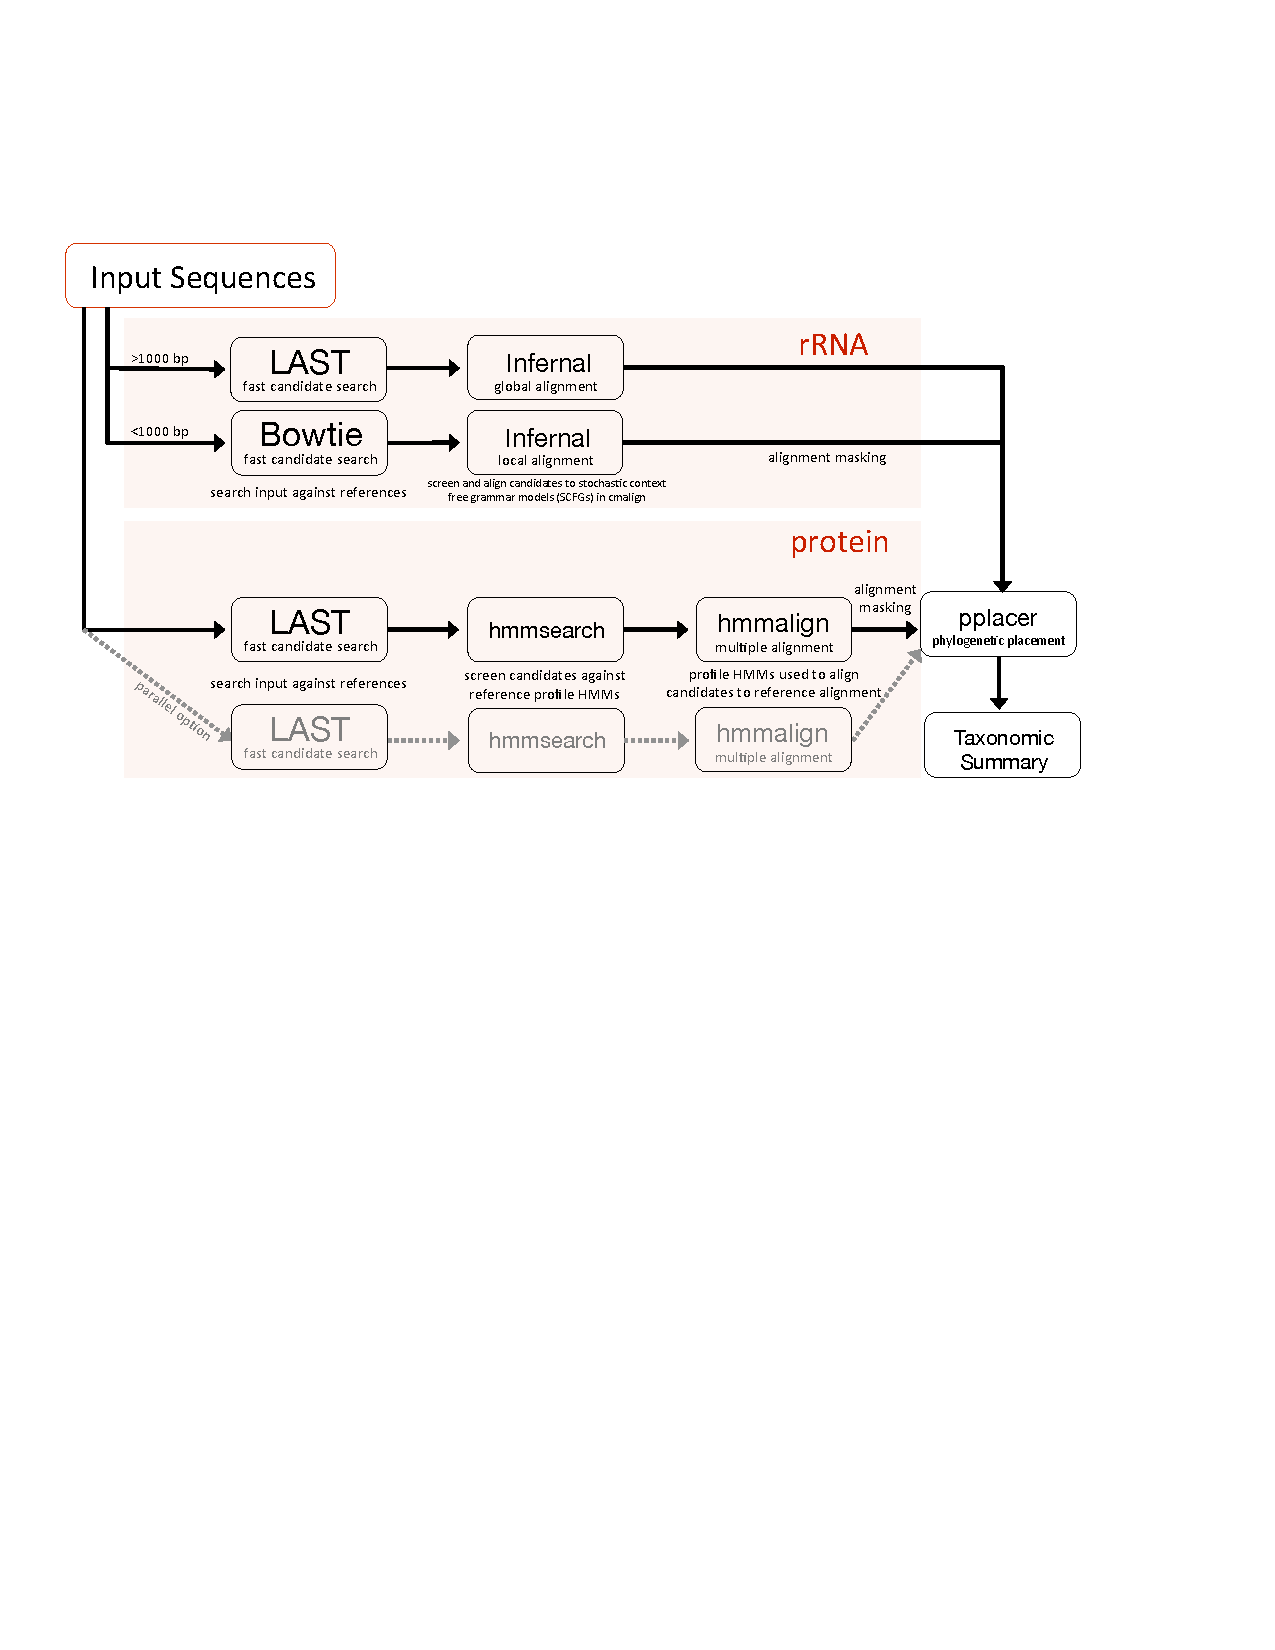
\includegraphics[trim=0 5.25in 0.5in 1.25in,clip,width=6.5in]{figures/Phylosift_overview_vector.pdf}
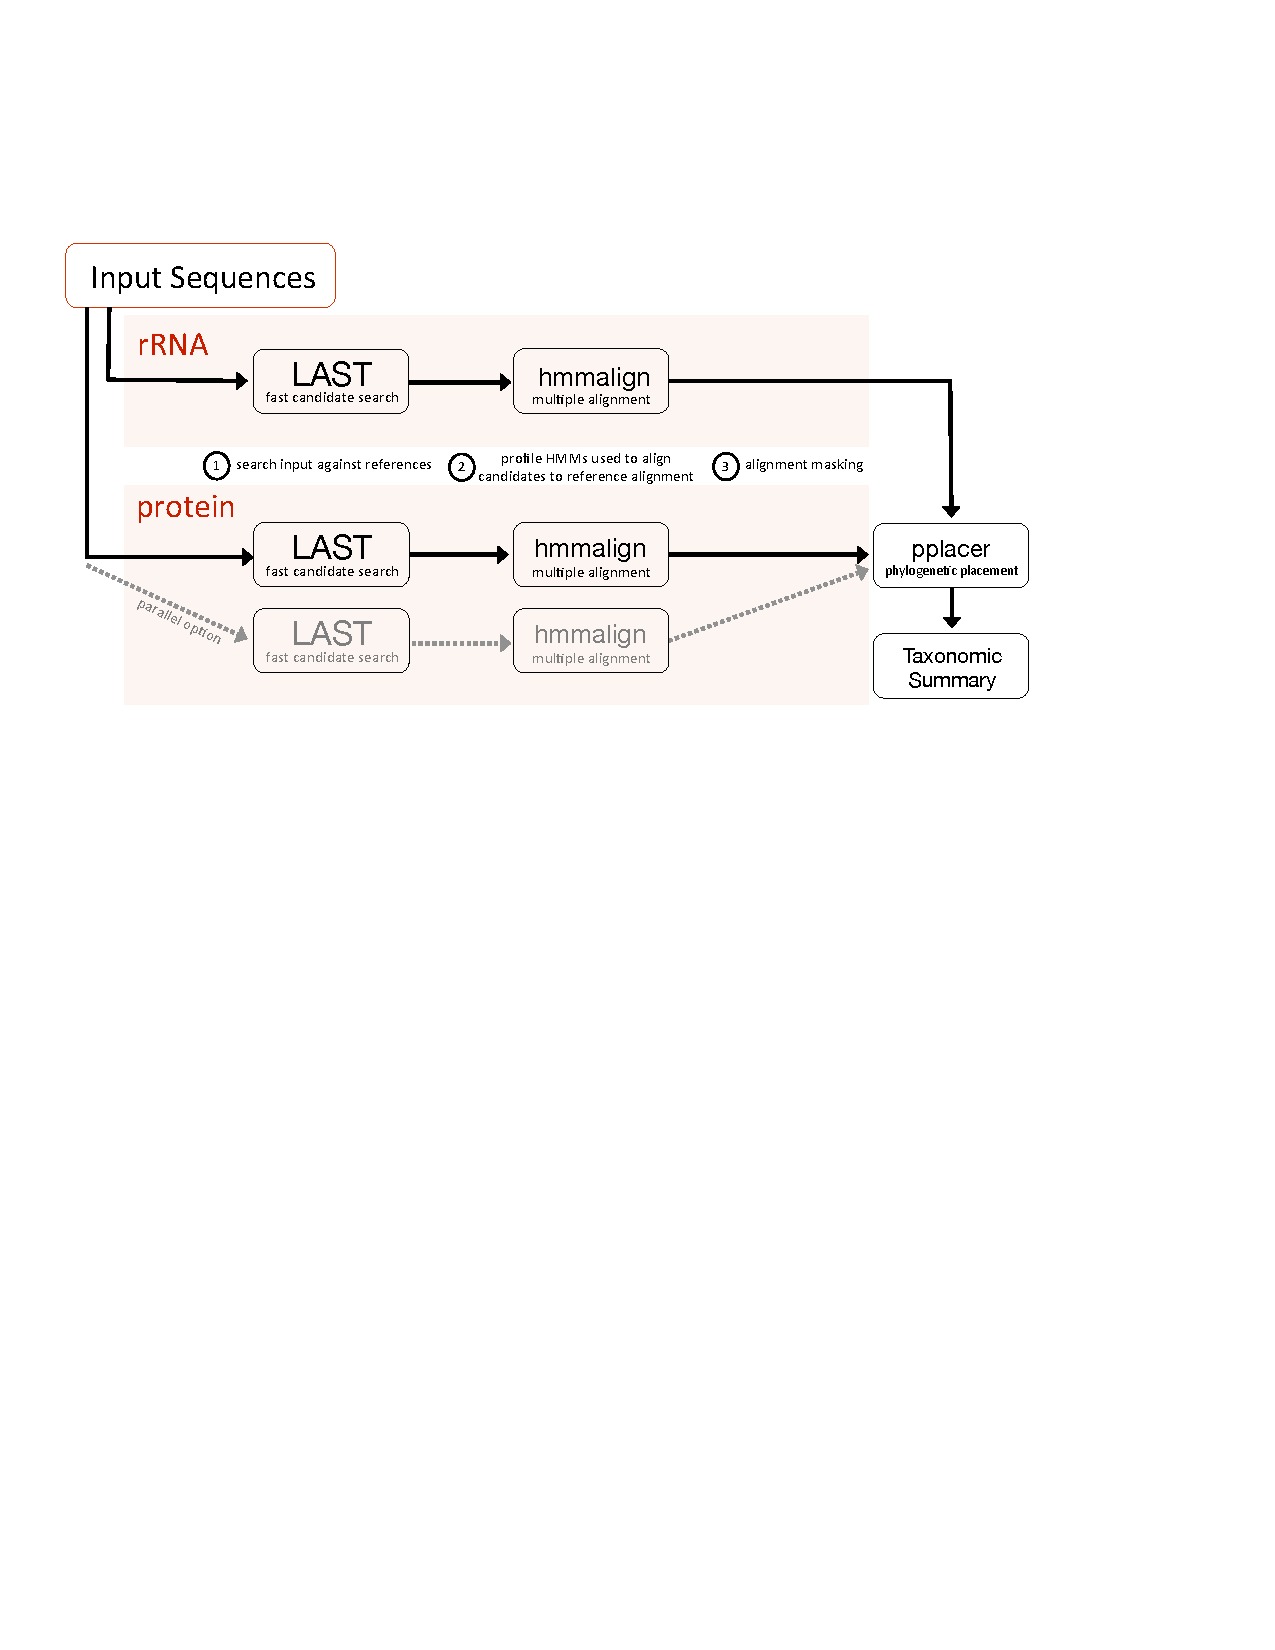
\includegraphics[width=6.5in]{figures/Phylosift_overview_oct2012_vector.pdf}
\end{center}
\caption{\textbf{PhyloSift client workflow.} This workflow is applied to the user's sequence data.}
\label{fig:overview}
\end{figure}

\begin{figure}[hp]
\begin{center}
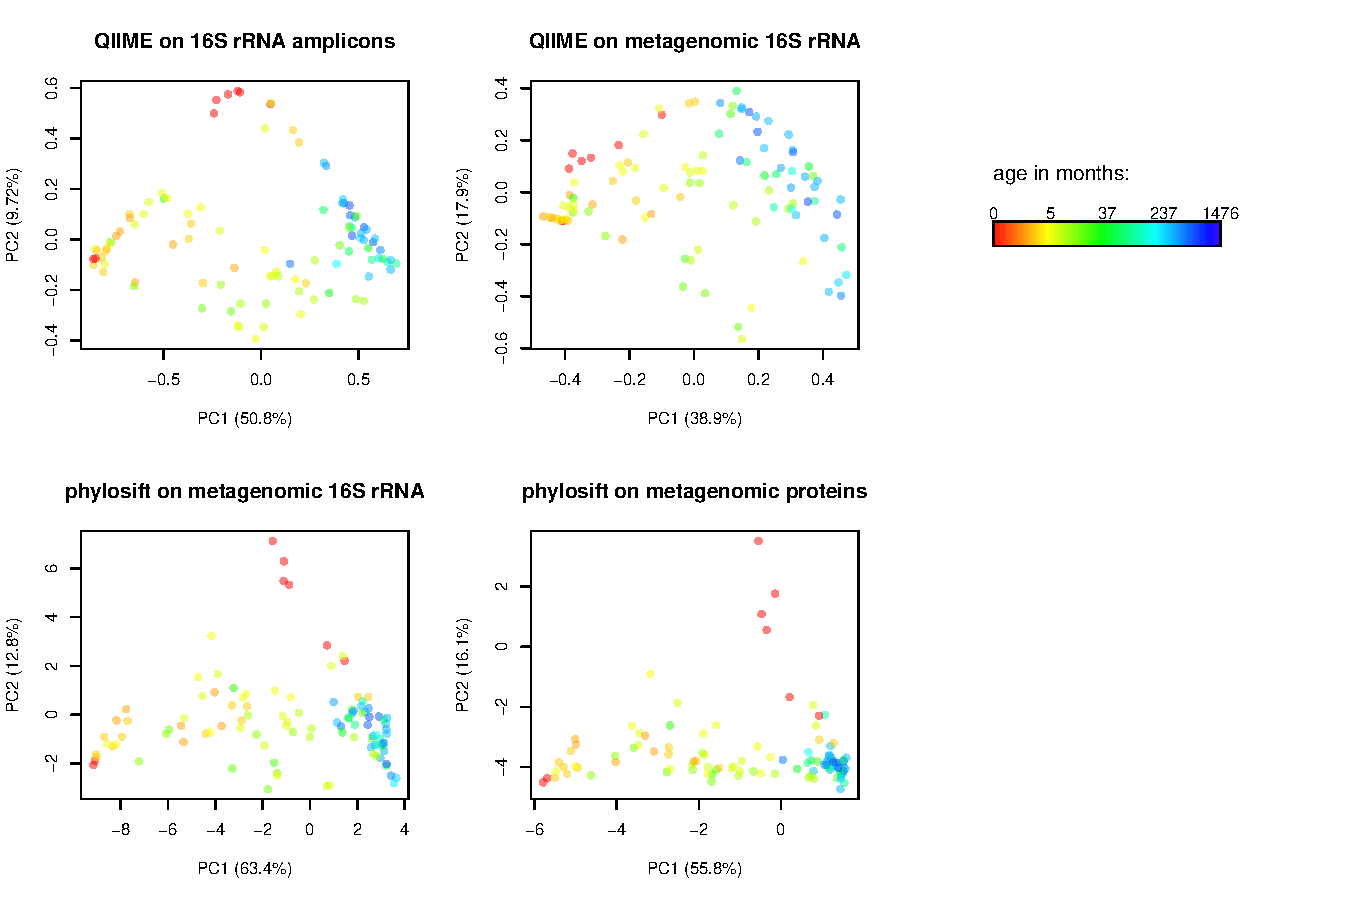
\includegraphics[width=6in]{figures/allofem.pdf}
\end{center}
\caption{\textbf{Comparison of QIIME PCA and edge PCA analysis of human fecal samples.} Samples from 107 (FIXME) individuals were analyzed by PCA to evaluate trends in community composition with respect to host age. 16S rDNA amplicon data and metagenomic data from the same samples was processed using QIIME and PhyloSift. QIIME analyzed the amplicon data (top left) and 16S rDNA reads extracted from the metagenomic data (top right) using a reference-based OTU picking strategy. PhyloSift analyzed the same metagenomic 16S rDNA reads (bottom left) and reads matching the 40 elite gene families (bottom right). Each PCA approach gives qualitatively similar results.}
\label{fig:agepca}
\end{figure}

\begin{figure}[hp]
\begin{center}
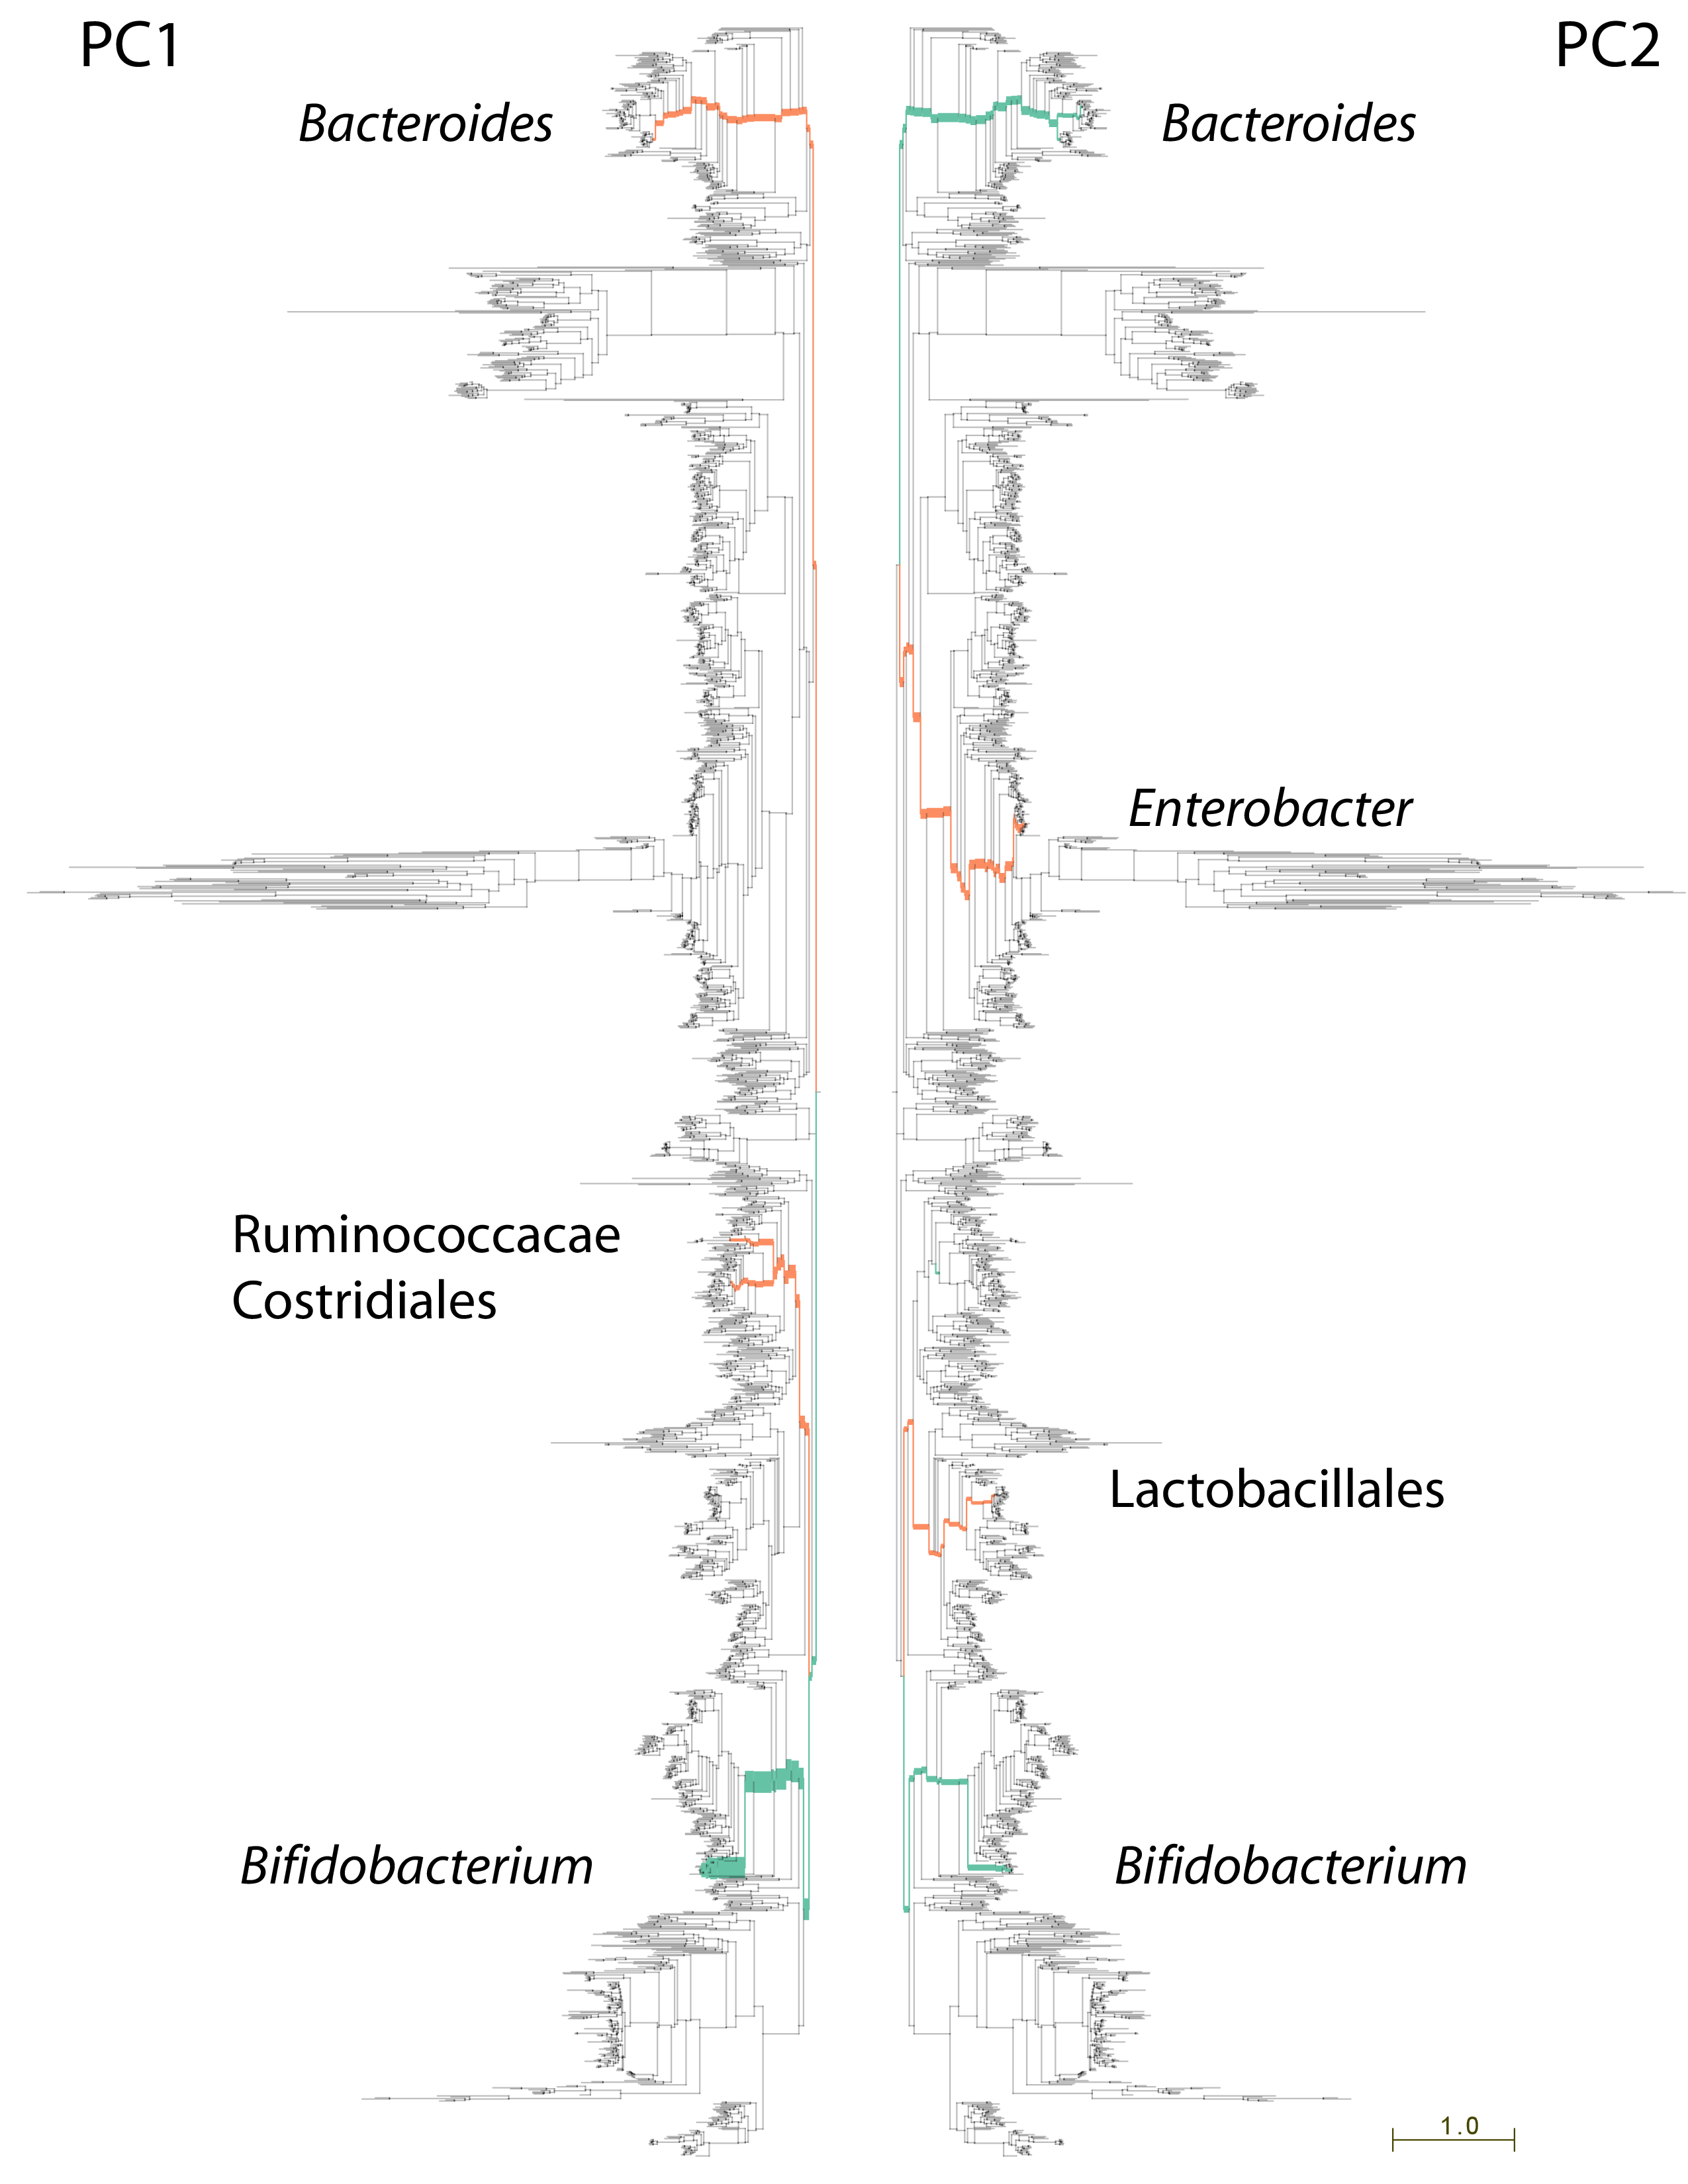
\includegraphics[width=6in]{figures/both_prettylike_b2b.pdf}
\end{center}
\caption{\textbf{Lineages contributing variation in human fecal sample community structure.} 110 metagenomic samples were processed using PhyloSift and their community composition compared using Edge PCA~\cite{Matsen2012}. Lineages that decrease in abundance along the principal component axis are shown in turquoise color, those increasing in abundance are shown in red. Edge width is proportional to the change in abundance. Remaining lineages in the phylogeny of bacteria, archaea, eukarya, and some viruses are shown in light gray. PC1 shown at left, PC2 at right.}
\label{fig:pcaphylo}
\end{figure}

\begin{figure}[hp]
\begin{center}
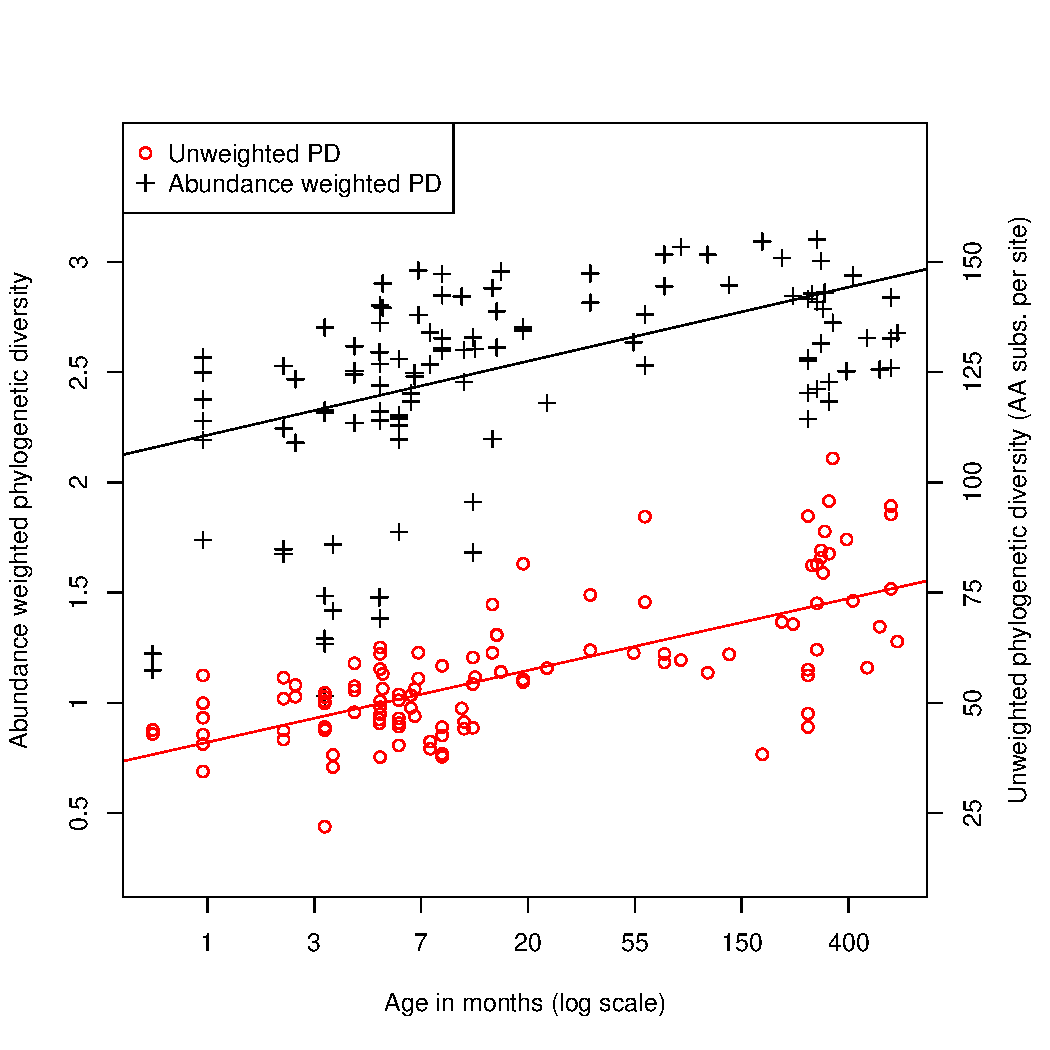
\includegraphics[width=4in]{figures/phylo_diversity.pdf}
\end{center}
\caption{\textbf{Relationship betwen fecal community phylogenetic diversity and host age.} 110 metagenomic samples were processed using PhyloSift and their phylogenetic diversity analyzed using two metrics. Unweighted phylogenetic diversity simply measures the total branch length of the reference tree covered by placed reads from a sample. Abundance-weighted phylogenetic diversity adjusts these values by the abundance of each lineage in the sample. In both cases, a log-linear relationship between host age and fecal community phylogenetic diversity can be observed.}
\label{fig:agediversity}
\end{figure}

\begin{figure}[hp]
\begin{center}
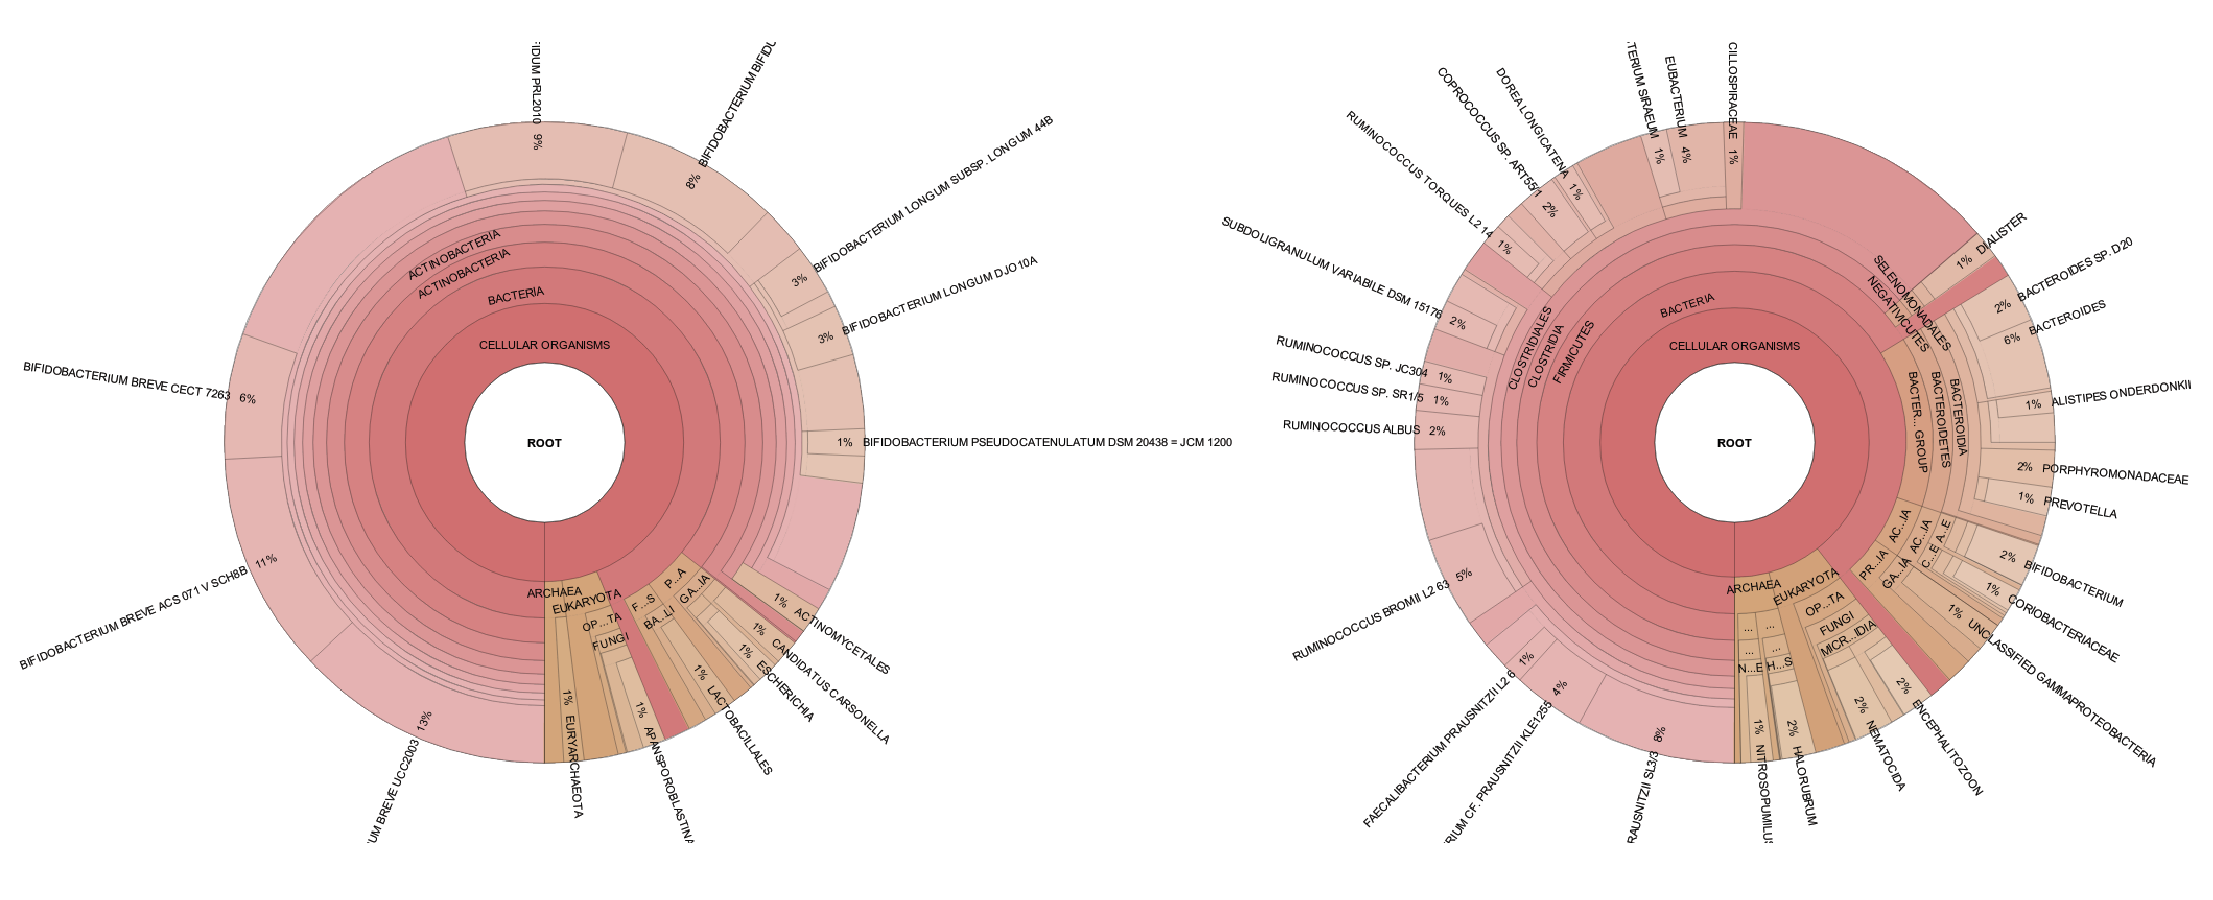
\includegraphics[width=6.5in]{figures/krona_two.pdf}
\end{center}
\caption{\textbf{Taxonomic visualization of two human gut samples.} Data analyzed by PhyloSift, visualized by Krona.}
\label{fig:kronaplots}
\end{figure}

\clearpage

\section*{Tables}


\clearpage

\end{document}

